\subsection{M.2.2 - Variazione pianificazione task completati}
\begin{figure}[H]
    \centering
    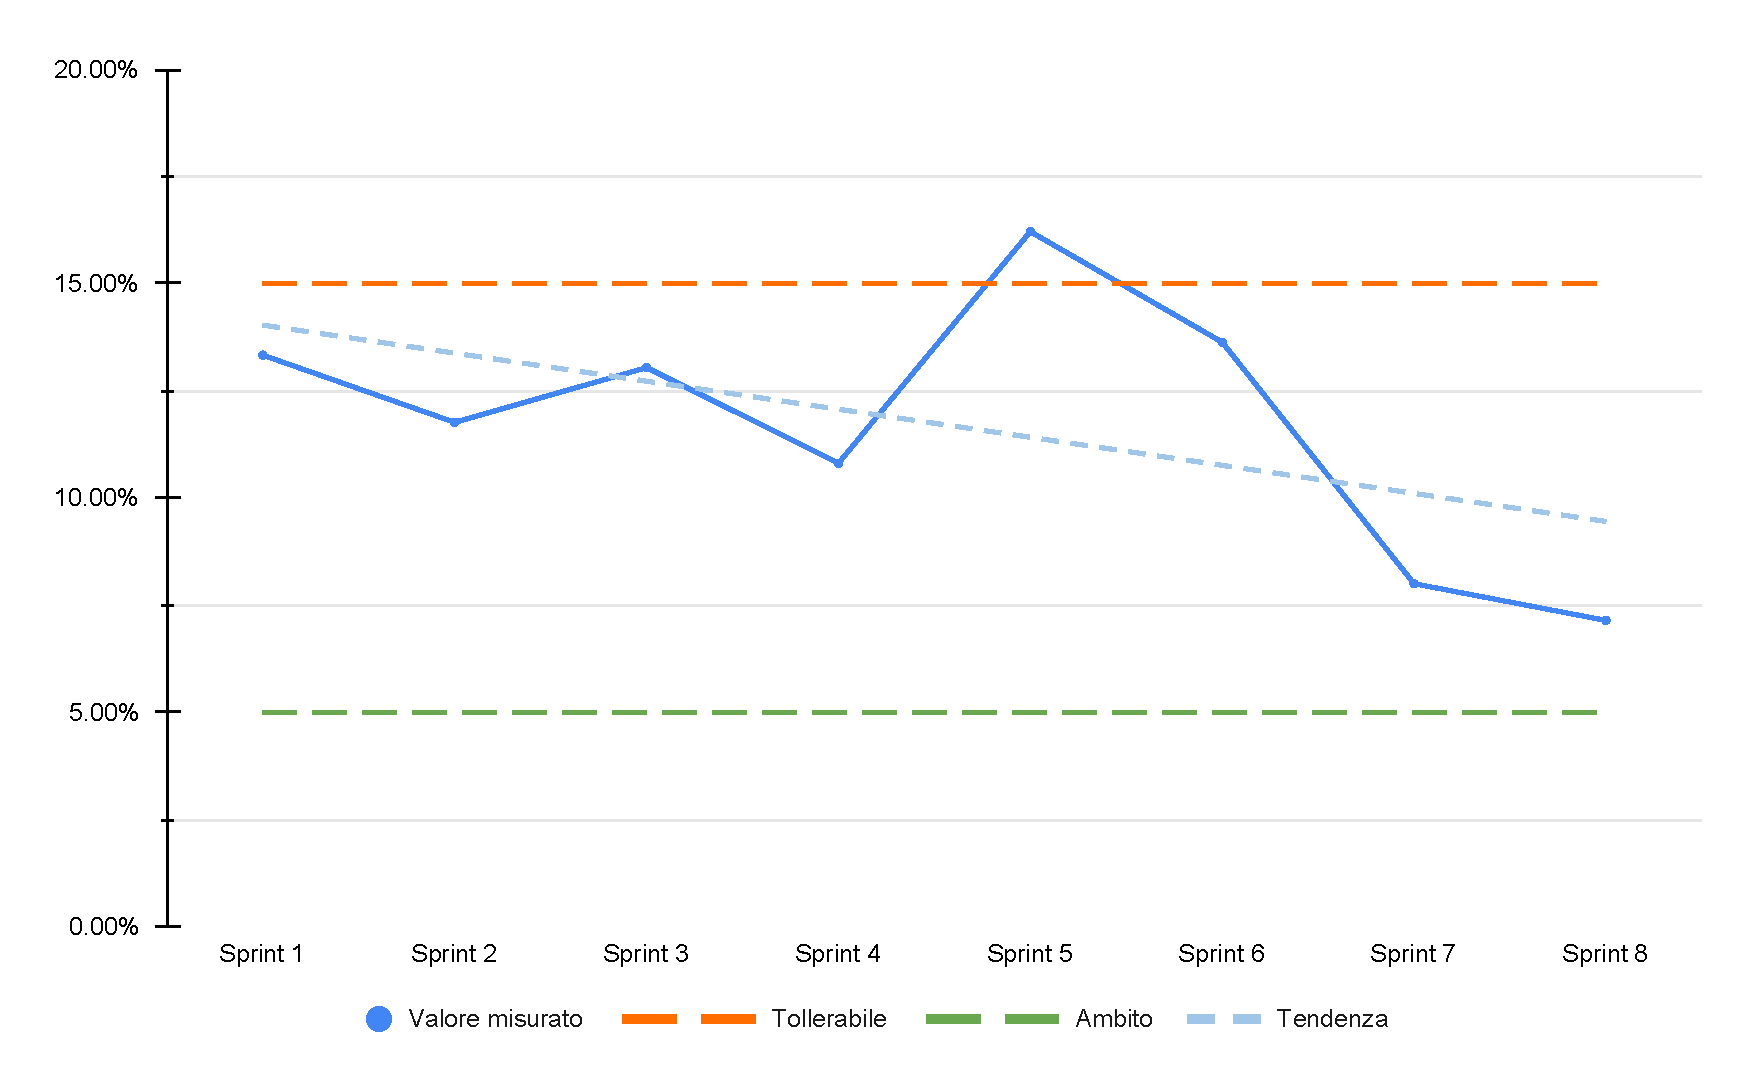
\includegraphics[width=0.8\textwidth]{assets/variazione_task_completati.pdf}
    \caption{M.2.2 - Variazione pianificazione task completati}
\end{figure}

\par Fino al quarto \glossario{sprint}, il team ha dovuto affrontare almeno un rischio inatteso.
Tuttavia, il numero di rischi non previsti è sempre stato inferiore rispetto alla soglia tollerabile.
Dallo \glossario{sprint} 5, invece, tutti i rischi che si sono verificati erano già stati analizzati e documentati nel \textit{Piano di Progetto}.
Questo ha permesso al team una migliore gestione del progetto. Di conseguenza, a partire dal settimo \glossario{sprint},
il gruppo ha deciso di abbassare il valore tollerabile a 1. L'obiettivo per le iterazioni successive, infatti, è mantenere il numero di rischi
inattesi quanto più stabile e prossimo al valore ambito.

\par Il gruppo ha mantenuto un sano equilibrio nel rapporto tra le attività pianificate ad inizio \glossario{sprint} e quelle non portate a termine all'interno del periodo determinato. Il risultato è indice di una pianificazione iniziale discretamente accurata, anche se non ottimale. Il picco in corrispondenza dello \glossario{sprint} 5 è dovuto alla sua durata minore, per cui la pianificazione iniziale non è stata bilanciata adeguatamente. A partire dalla misura successiva si è tuttavia riconsiderato il carico di lavoro, rientrando nel range di tollerabilità.